This chapter shows the important details of the Smart Shelf implementation. 
The system of the Smart Shelf itself consists of three main components. 
The backend server with a MySQL database, a webapp served by the backend and Smart Shelf itself with an Arduino as main microcontroller connected to some electronic components placed in the drawers. 
Basically, the Smart Shelf is contained of several Smart Drawers. 
These components and how they communicate with each other are described in the following. 
%
\begin{figure*}
	\centering
	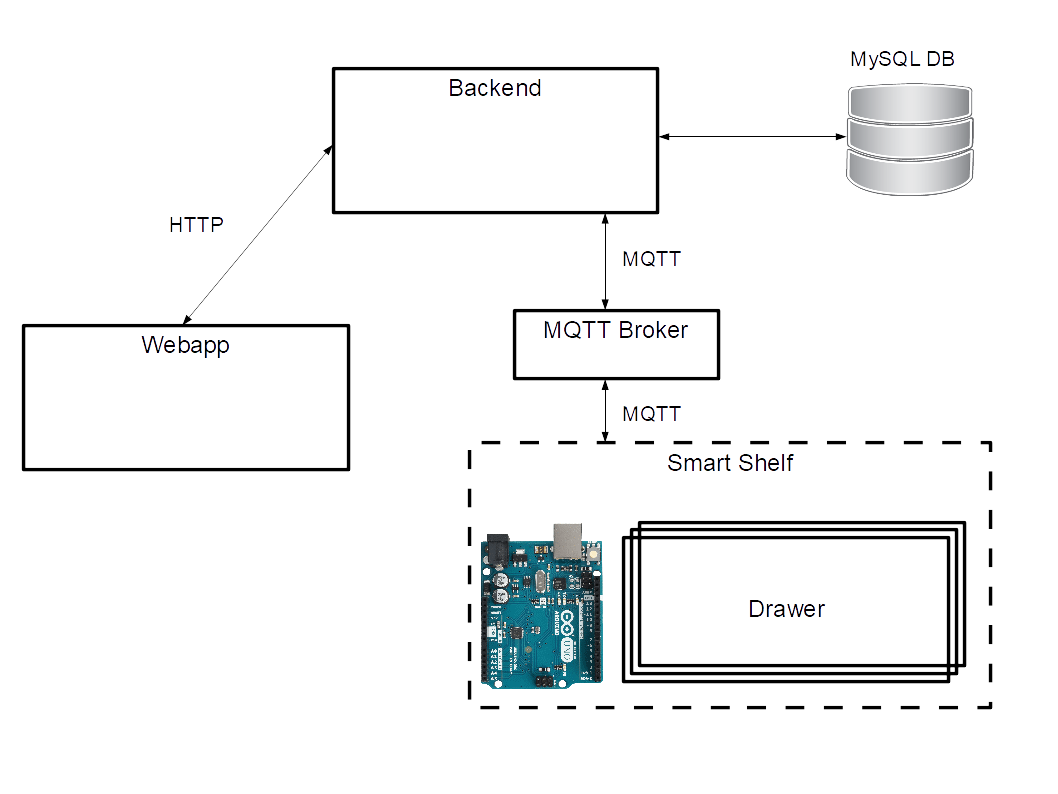
\includegraphics[width=1.3\columnwidth]{figures/infrastructure-smartshelf-white.png}
	\caption{Infrastructure of the Smart Shelf system}~\label{fig:infrastructure}
\end{figure*}
%

\subsection{Backend}
For the backend implementation the Spring framework is used \cite{springframework}. 
This enables to build a lightweight backend server that can serve web pages, a REST API and can connected to a MQTT\footnote{Abbr. Message Queuing Telemetry Transport Protocol} broker. 
The communication between backend and Arduino with MQTT is explained in section \ref{sec:communciation} in detail. 
To serve the webapp the backend implements several REST Services which can be consumed via HTTP. 
Some of this services produce the different web pages for the webapp. 
Others produce just data to keep the information in the webapp up to date. 

As mentioned before the backend keeps the state of the whole system. 
For that it implements some queues for all current search queries and has a connection to a MySQL database with all the essential data needed for the Smart Shelf. 
The database contains for example all items contained in the shelf, in which drawer these items are and what boxes are there. 
Additional information like the amount of different items are stored, too. 
To enable the PMS the backend implements also some services to mark an item as out of stock and to send an email to defined operators as notification. 
These operators can subsequently order supply for the appropriate items. 
In addition to the sent notification the backend sends a command to the Arduino to switch on the red LED on that drawer. 
This signals directly to each user that this drawer is empty. 

To use more of the capabilities the visual feedback provided via the LEDs on the drawers the Smart Shelf implements a so called service mode. 
This mode can be started from the webapp. 
After started the backend checks the state of all drawers and send the appropriated commands to the Arduino to switch on the correct LED on all drawers. 
As mentioned before there is a mapping between the colours of the LED and the amount of items in a drawer. 
Blue colour signals that the amount of items in that drawer is above a defined threshold. 
Yellow colour indicates that the amount is below the threshold and red visualizes that this drawer is empty. 

\subsection{Communication}\label{sec:communciation}
For the communication between Arduino and backend the lightweight M2M\footnote{Abbr. Machine-to-Machine} communication protocol MQTT was chosen. 
MQTT works with the publish and subscribe pattern. 
There is a central broker where clients can subscribe topics. 
Additionally, clients can publish messages to different topics. 
If a client subscribed the topic under which a message is published, the client will receive it \cite{standard2014mqtt}. 
For further information about this protocol check \cite{standard2014mqtt}. 

With MQTT a bidirectional connection can be established between backend and Arduino. 
Primary, the backend send commands to the Arduino which LEDs the Arduino should switch on or off. 
But additionally, the Arduino send in a defined interval the measured weights of items contained in different drawers. 
How the weight measurement is done is explained in following chapters. 

\subsection{Control System of Drawers}
\subsection{Shelf Control System}
The whole concept of smart shelf follows a IoT principle. According to previously mentioned Publish/Subscribe patter the Arduino which is the main controller of the smart shelf is subscribed with some topic in the MQTT broker. The server itself publish topic based with some name so that Arduino can receive the user command from the MQTT broker. After receiving the information Arduino parse the JSON text and invoke command to glow any led based on the server side information. Similarly, The reading from sensor send to the back end in the same way the we receive information from backend, but this time the Web-app act as a subscriber to topics and Arduino publishes on that topics.  The communication tool and hardware used for communicating with server is Ethernet communication which solely operated by the ethernet card Arduino Ethernet Shied.
\paragraph*{Communication Algorithm: }


\subsection{Smart Drawer}
To fulfil  the purpose of prototype and reduce the cost of implementation we implemented two fully featured drawers that includes weight sensing and visual output and four basic drawers that consists of only visual output modules.
The fully featured drawer contain one load cell(Model), the load cell is employed to measure the pressure of equipments that is generally stored in the drawers. The signal of the load cell is then amplified via an amplifier to feed into the Arduino. Moreover, The visual feed back module is made of three LEDs that are operated by the Arduino. Similarly, the basic drawers work based on same principle; however the there is no weight sensing technique. The schematic  \ref{fig:example_circuit}  shows the hardware implementation of the full featured drawer. Also the figure  \ref{fig:example_drawer} shows the visual demonstration of drawer. The transparent plate attached with the load cell is used to place equipment to over it to measure the wight. The load cell below measure the pressure due to the placement of equipment over the visible board. 
%
\begin{figure}
	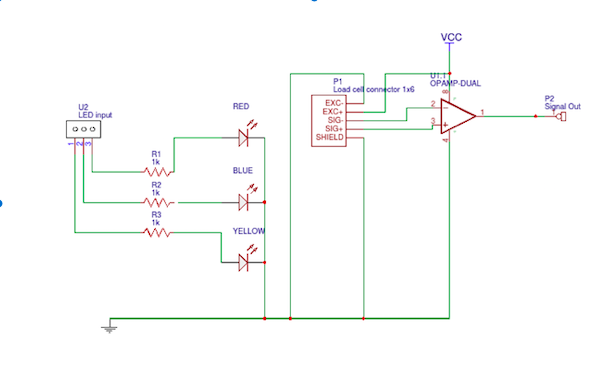
\includegraphics[width=1\columnwidth]{figures/drawer_circuit}
	\caption{Circuit diagram of smart drawer}~\label{fig:example_circuit}
\end{figure}
\begin{figure}
	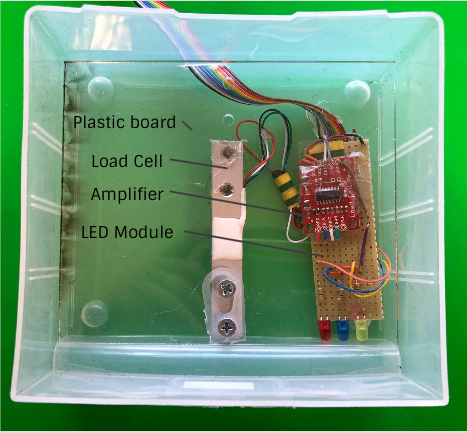
\includegraphics[width=1\columnwidth]{figures/drawer.png}
	\caption{Hardware configuration of a smart drawer}~\label{fig:example_drawer}
\end{figure}
%
\\

\subsection{Webapp}
To control the Smart Shelf a webapp is served by the backend. 
This webapp can be opened via an URL from almost every browser which is connected to the network the backend is in. 
Implementing the user interface as webapp brings the advantage of platform independence. 
It can be used form a Android or iOS phone as well as with computer. 

Figure \ref{fig:webapp-mainpage} shows the main page of the user interface. 
%
\begin{figure*}
	\centering
	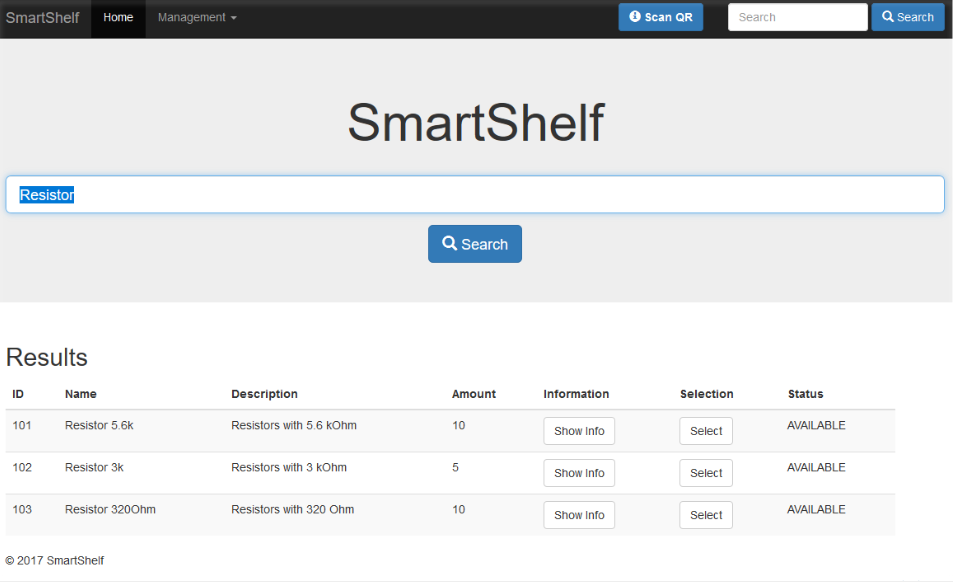
\includegraphics[width=1.3\columnwidth]{figures/ui-mainpage.png}
	\caption{Mainpage of the webapp}~\label{fig:webapp-mainpage}
\end{figure*}
%
The main function of the system is to make it easy searching for a item in the shelf. 
Therefore, a big search field can directly be seen at the main page. 
Inserting there the name of the searched item results in a list of items matching the inserted name. 
Additionally, all LEDs of the drawers which contain the displayed items in the webpage will be turned on. 
By using the "Select"-button for the item to choice all LEDs will be switched off except the selected one. 
With this functionality the user can easily find the search item without scanning the all drawers for the specific name. 

To get more information about an item one can uses the data sheet provided by the webapp. 
This can directly reached from the search result, also seen in figure \ref{fig:webapp-mainpage}, or by scanning the QR-Code mounted on the appropriate drawer. 
The QR-Code brings the advantage that if a user need more information about a specific item and is standing right in front of the shelf he/she doesn't have to search again and afterwards select the data sheet. 
The data sheet can easily get by scanning the QR-Code with the smart phone which used to operate the webapp. 
As mentioned before the QR-Code encodes the ID of the drawer. 
By scanning this ID is decoded, send to the backend which responds with the needed information about that drawer to visualize the correct data sheet. 